\documentclass[12pt]{article}

\usepackage[font=footnotesize]{caption}
\usepackage{float}
\usepackage{epsf}
\usepackage{epsfig}
\usepackage{subfigure}
% \usepackage{subfig}
\usepackage{latexsym}
%\usepackage{algorithm}
%\usepackage[noend]{algorithmic}
% \usepackage{color}
\usepackage{color, colortbl}
\usepackage{wrapfig}
\usepackage{topcapt}
\usepackage{multirow}
\usepackage{tabularx}
\usepackage{hyperref}
\usepackage{xcolor}
\usepackage{mdwlist}
\usepackage{pdfpages} 

%\usepackage{color}
\newcommand{\lc}[1]{\textcolor{blue}{#1}}


\usepackage{amsmath, amsfonts, amssymb}
\usepackage[hmargin=1in,vmargin=1.2in]{geometry}
\usepackage{url}
\usepackage{multirow}
\usepackage[ruled,noline,linesnumbered]{algorithm2e}
\usepackage[bottom]{footmisc}
\usepackage{afterpage}
%\usepackage[caption=false]{caption}
\usepackage{eurosym}
\usepackage{enumitem}
% \usepackage{soul}
\usepackage{fancyhdr}
\usepackage{dashrule}
% \usepackage[stable]{footmisc}
% \usepackage{placeins}
% \setitemize{noitemsep,topsep=0pt,parsep=0pt,partopsep=0pt}
% \usepackage[utf8]{inputenc}
\usepackage{gensymb}

\widowpenalty=1000
\clubpenalty=1000

\input{epsf}

\def\nas{{NASA\ }}
\def\nase{{NASA}}
\def\esa{{ESA\ }}
\def\esae{{ESA}}
\def\inst{{NASA Ames Research Center\ }}
\def\inste{{NASA Ames Research Center}}
\def\univ{{UPorto\ }}
\def\unive{{UPorto}}
\def\soc{{SOCIB\ }}
\def\soce{{SOCIB}}
\def\vig{{UVigo\ }}
\def\vige{{UVigo}}
\def\ldeo{{LDEO\ }}
\def\ldeoe{{LDEO}}
\def\ls{{LSTS\ }}
\def\lse{{LSTS}}
\def\sml{{SmallSat\ }}
\def\smle{{SmallSat}}
\def\mba{{MBARI\ }}
\def\mbae{{MBARI}}
\def\rpe{{REP}}
\def\rp{{REP\ }}
\def\org{{SIFT\ }}
\def\orge{{SIFT}}
\def\pro{{\textmd{METEOR\ }}}
\def\proe{{\textmd{METEOR}}}
\def\kck{{Keck Foundation\ }}
\def\kcke{{Keck Foundation}}


\newlength{\doublespacelength}
\setlength{\doublespacelength}{\baselineskip}
\addtolength{\doublespacelength}{0.5\baselineskip}
\newcommand{\doublespace}{\setlength{\baselineskip}{\doublespacelength}}

\newlength{\singlespacelength}
\setlength{\singlespacelength}{\baselineskip}
\newcommand{\singlespace}{\setlength{\baselineskip}{\singlespacelength}}


\newlength{\savedspacing}
\newcommand{\savespacing}{\setlength{\savedspacing}{\baselineskip}}
\newcommand{\restorespacing}{\setlength{\baselineskip}{\savedspacing}}

\setlength{\parskip}{0pt}
\setlength{\parsep}{0pt}
\setlength{\headsep}{0pt}
\setlength{\topskip}{0pt}
\setlength{\topmargin}{0pt}
\setlength{\topsep}{0pt}
\setlength{\partopsep}{0pt}

\newcommand{\kc}[1]{{\color{red}{#1}}}
\newcounter{quotenumber}

\newenvironment{numquote}{%
    \begin{enumerate}%
     \setcounter{enumi}{\value{quotenumber}}%
     \color{darkgray}
    \item \begin{quote}%
}{%
    \end{quote}%
    \setcounter{quotenumber}{\value{enumi}}
    \end{enumerate}%
}%

\makeatletter
\def\myitem{%
   \@ifnextchar[ \@myitem{\@noitemargtrue\@myitem[\@itemlabel]}}
\def\@myitem[#1]{\item[#1]\mbox{}}
\makeatother
\definecolor{Gray}{gray}{0.6}


\newcommand\blankpage{%
    \null
    \thispagestyle{empty}%
    \addtocounter{page}{-1}%
    \newpage}

\setcounter{secnumdepth}{0} 



\fancyhead[L]{}% empty left
\fancyhead[R]{ % right
  
\includegraphics[width=0.95in,height=0.45in]{fig/uporto.png}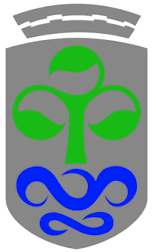
\includegraphics[height=0.45in]{fig/vigo.png}
\includegraphics[height=0.45in]{fig/ldeo.jpg}
}
\pagestyle{fancy}


\begin{document}

\vspace*{1cm}
\begin{center}
  {\large \bf{\proe}: A Portable Robotic Observatory for Diagnosing Coastal Ocean Health for Human Well Being}\\
% Coordinated Oceanographic Observations
  \today
\end{center}

\vspace*{0.5cm}

\fcolorbox{black}[HTML]{E9F0E9}{\parbox{6.0in}{%

    Our oceans host enormous biodiversity, provide multiple ecosystem
    services, sustain vibrant economies, and play a significant role
    in climate regulation, but are threatened by human activity and
    climate change.
    % Our oceans, which host enormous biodiversity, providing multiple
    % ecosystem services, sustain a vibrant economy, and play a
    % significant role in climate regulation, are in trouble.
    We need a \textbf{sustained}, \textbf{persistent}, and
    \textbf{affordable} presence there to help us understand and
    monitor how key processes such as acidification, hypoxia, toxic
    blooms, pollution and erosion (amongst others) are impacting
    global ocean sustainability and
    stewardship. % Traditional ship and remote-sensing methods
    % neither prove cost-effective nor provide assimilated real-time
    % information at appropriate human relevant scales.
    In coastal regions, this is especially important, because these
    areas mediate most of the interactions between a significant
    percentage of the world population and the oceans. An integrative
    sea management approach and the protection of natural capital and
    marine ecosystem resources can only be achieved with the help of
    coordinated observations from space, aerial, surface and
    underwater robots guided by Artificial Intelligence (AI) while
    providing continual and reliable oceanographic data.}}

\subsection{The Idea}

% \begin{figure}[!t]
%   \centering
%   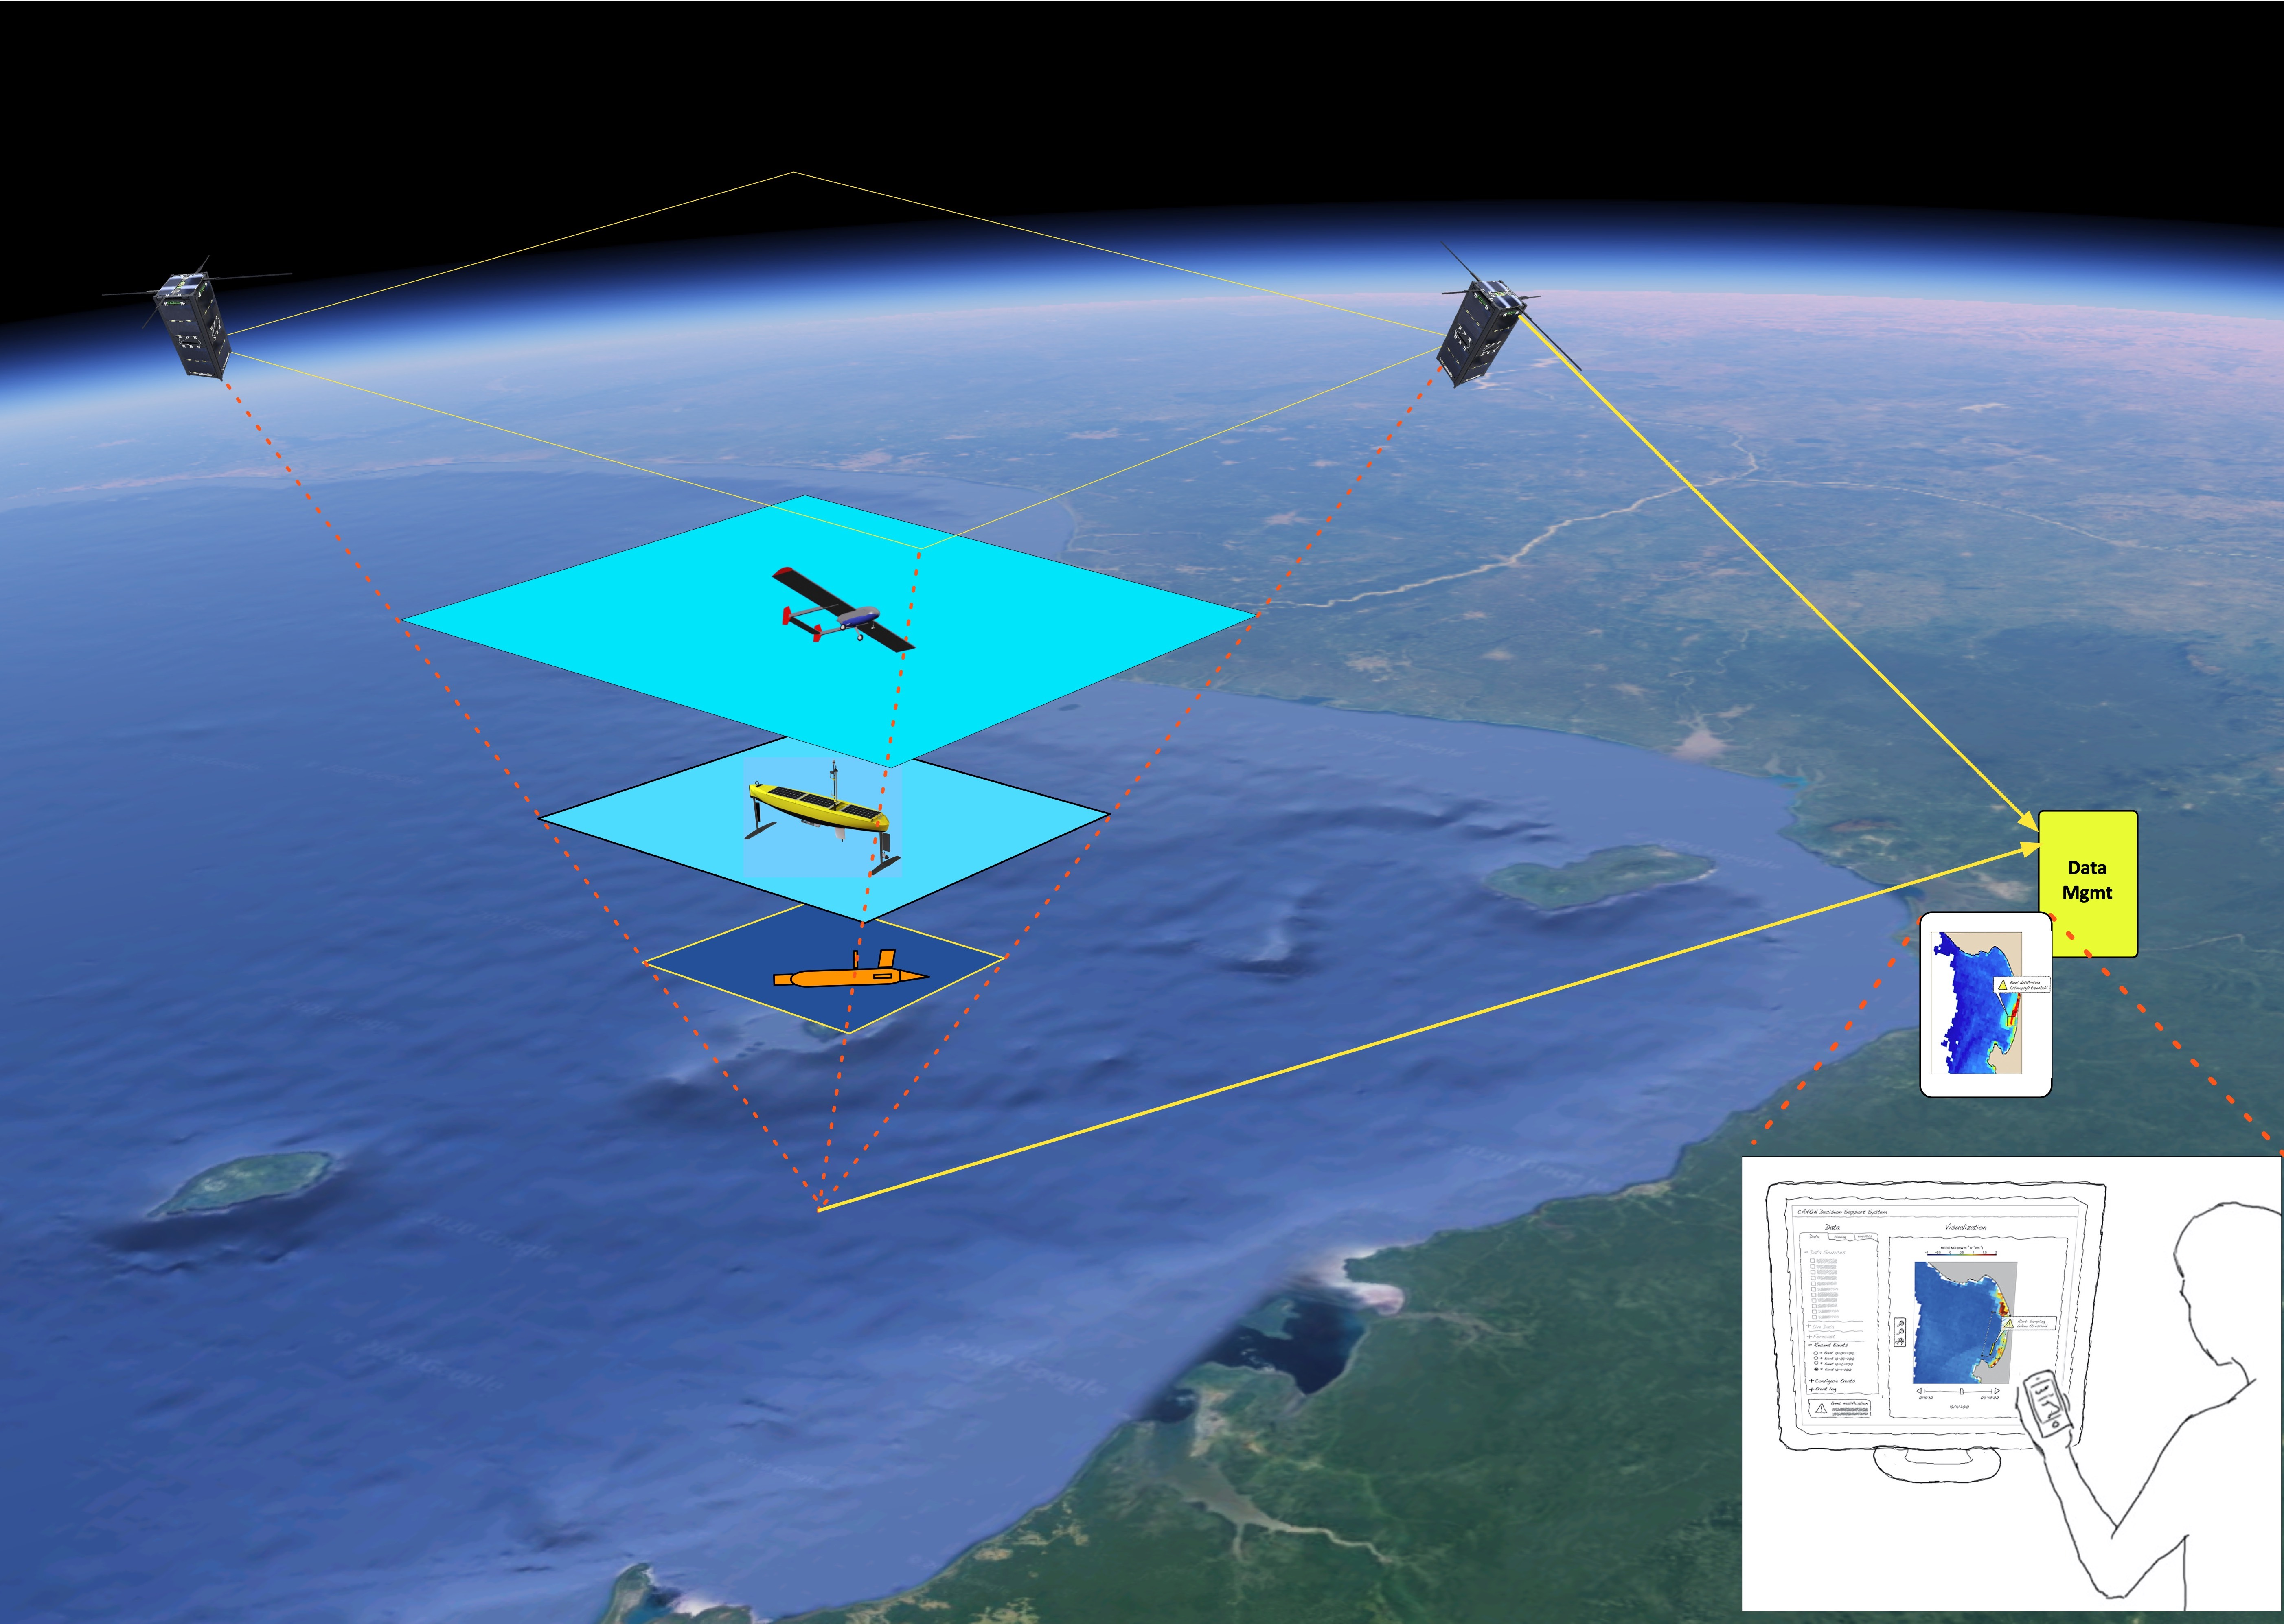
\includegraphics[scale=0.06]{fig/procopio-ensemble.jpg}
%   \caption{\pro is an ensemble of small satellites, aerial, surface
%       and underwater vehicles to observe the coastal ocean over
%       sustained periods of time.}
%   \label{fig:procop}
% \end{figure}

Urban population growth has exacerbated the pressures on the coastal
ecosystem along what is now called the ``Urban Sea''. Even as these
waters are vital to the economic and general well-being of more than
800 million people, they are increasingly threatened by pollution and
anthropogenic discharge. Resultant toxic blooms and oxygen depletion
have had deleterious effects on fisheries and other critical resources
that coastal populations depend on, while also impacting human
health. Furthermore, extreme weather events induced by climate change
will only hasten the worsening of water quality of Urban Seas because
of enhanced runoff, coastal erosion and storm surges.

Many large telescopes point toward the heavens, but no such
observational system exists for looking at and into our oceans. We aim
to change that. Our mission is to build a portable, rapidly deployable
anywhere, robotic observatory for observing and managing the health of
our endangered coastal
waters % using Small Satellites, unmanned aerial,
% surface and underwater vehicles
(Fig. \ref{fig:mega-cities}).

\pro (A Portable Robotic Observatory for Coordinated Oceanographic
Observations) will be a modular system with bespoke approaches related
to water quality in the world's coastal zones with mega-cities. It
will provide actionable information for water quality measurements for
lay persons who can obtain near real-time (hours) data visualized at
spatial and temporal scales to provide accurate information to deal
with coastal pollution, erosion, toxic waters and sediment laden
plumes.

Stakeholders across governments, industry, science, nonprofits and
citizenry will make use of layered views ranging from basic visuals
for lay users to the complex queries needed for effective management
of resources and increased scientific knowledge.


% In particular, coastal zone human habitation has a large and direct
% impact because of interactions between humankind and the oceans; this
% is particularly so with large populations in mega-cities.  Among human
% generated activities, pesticides and nutrients used in agriculture end
% up in the coastal waters, resulting in oxygen depletion that affects
% marine plants and shellfish.  Factories and industrial facilities
% discharge sewage and other runoff while oil spills from ships and
% water-sewage treatment plants discharge toxic material polluting the
% oceans.  Air pollution results in toxic contaminants and nutrients
% that enter coastal areas and oceans.  Invasive species such as toxic
% algae, cholera, and countless plants and animals enter harbor waters
% and disrupt the ecological balance. Typically such discharges occur
% near large human habitats which are also a source of recreation and
% sea food.


\begin{figure}[H]
  \centering
  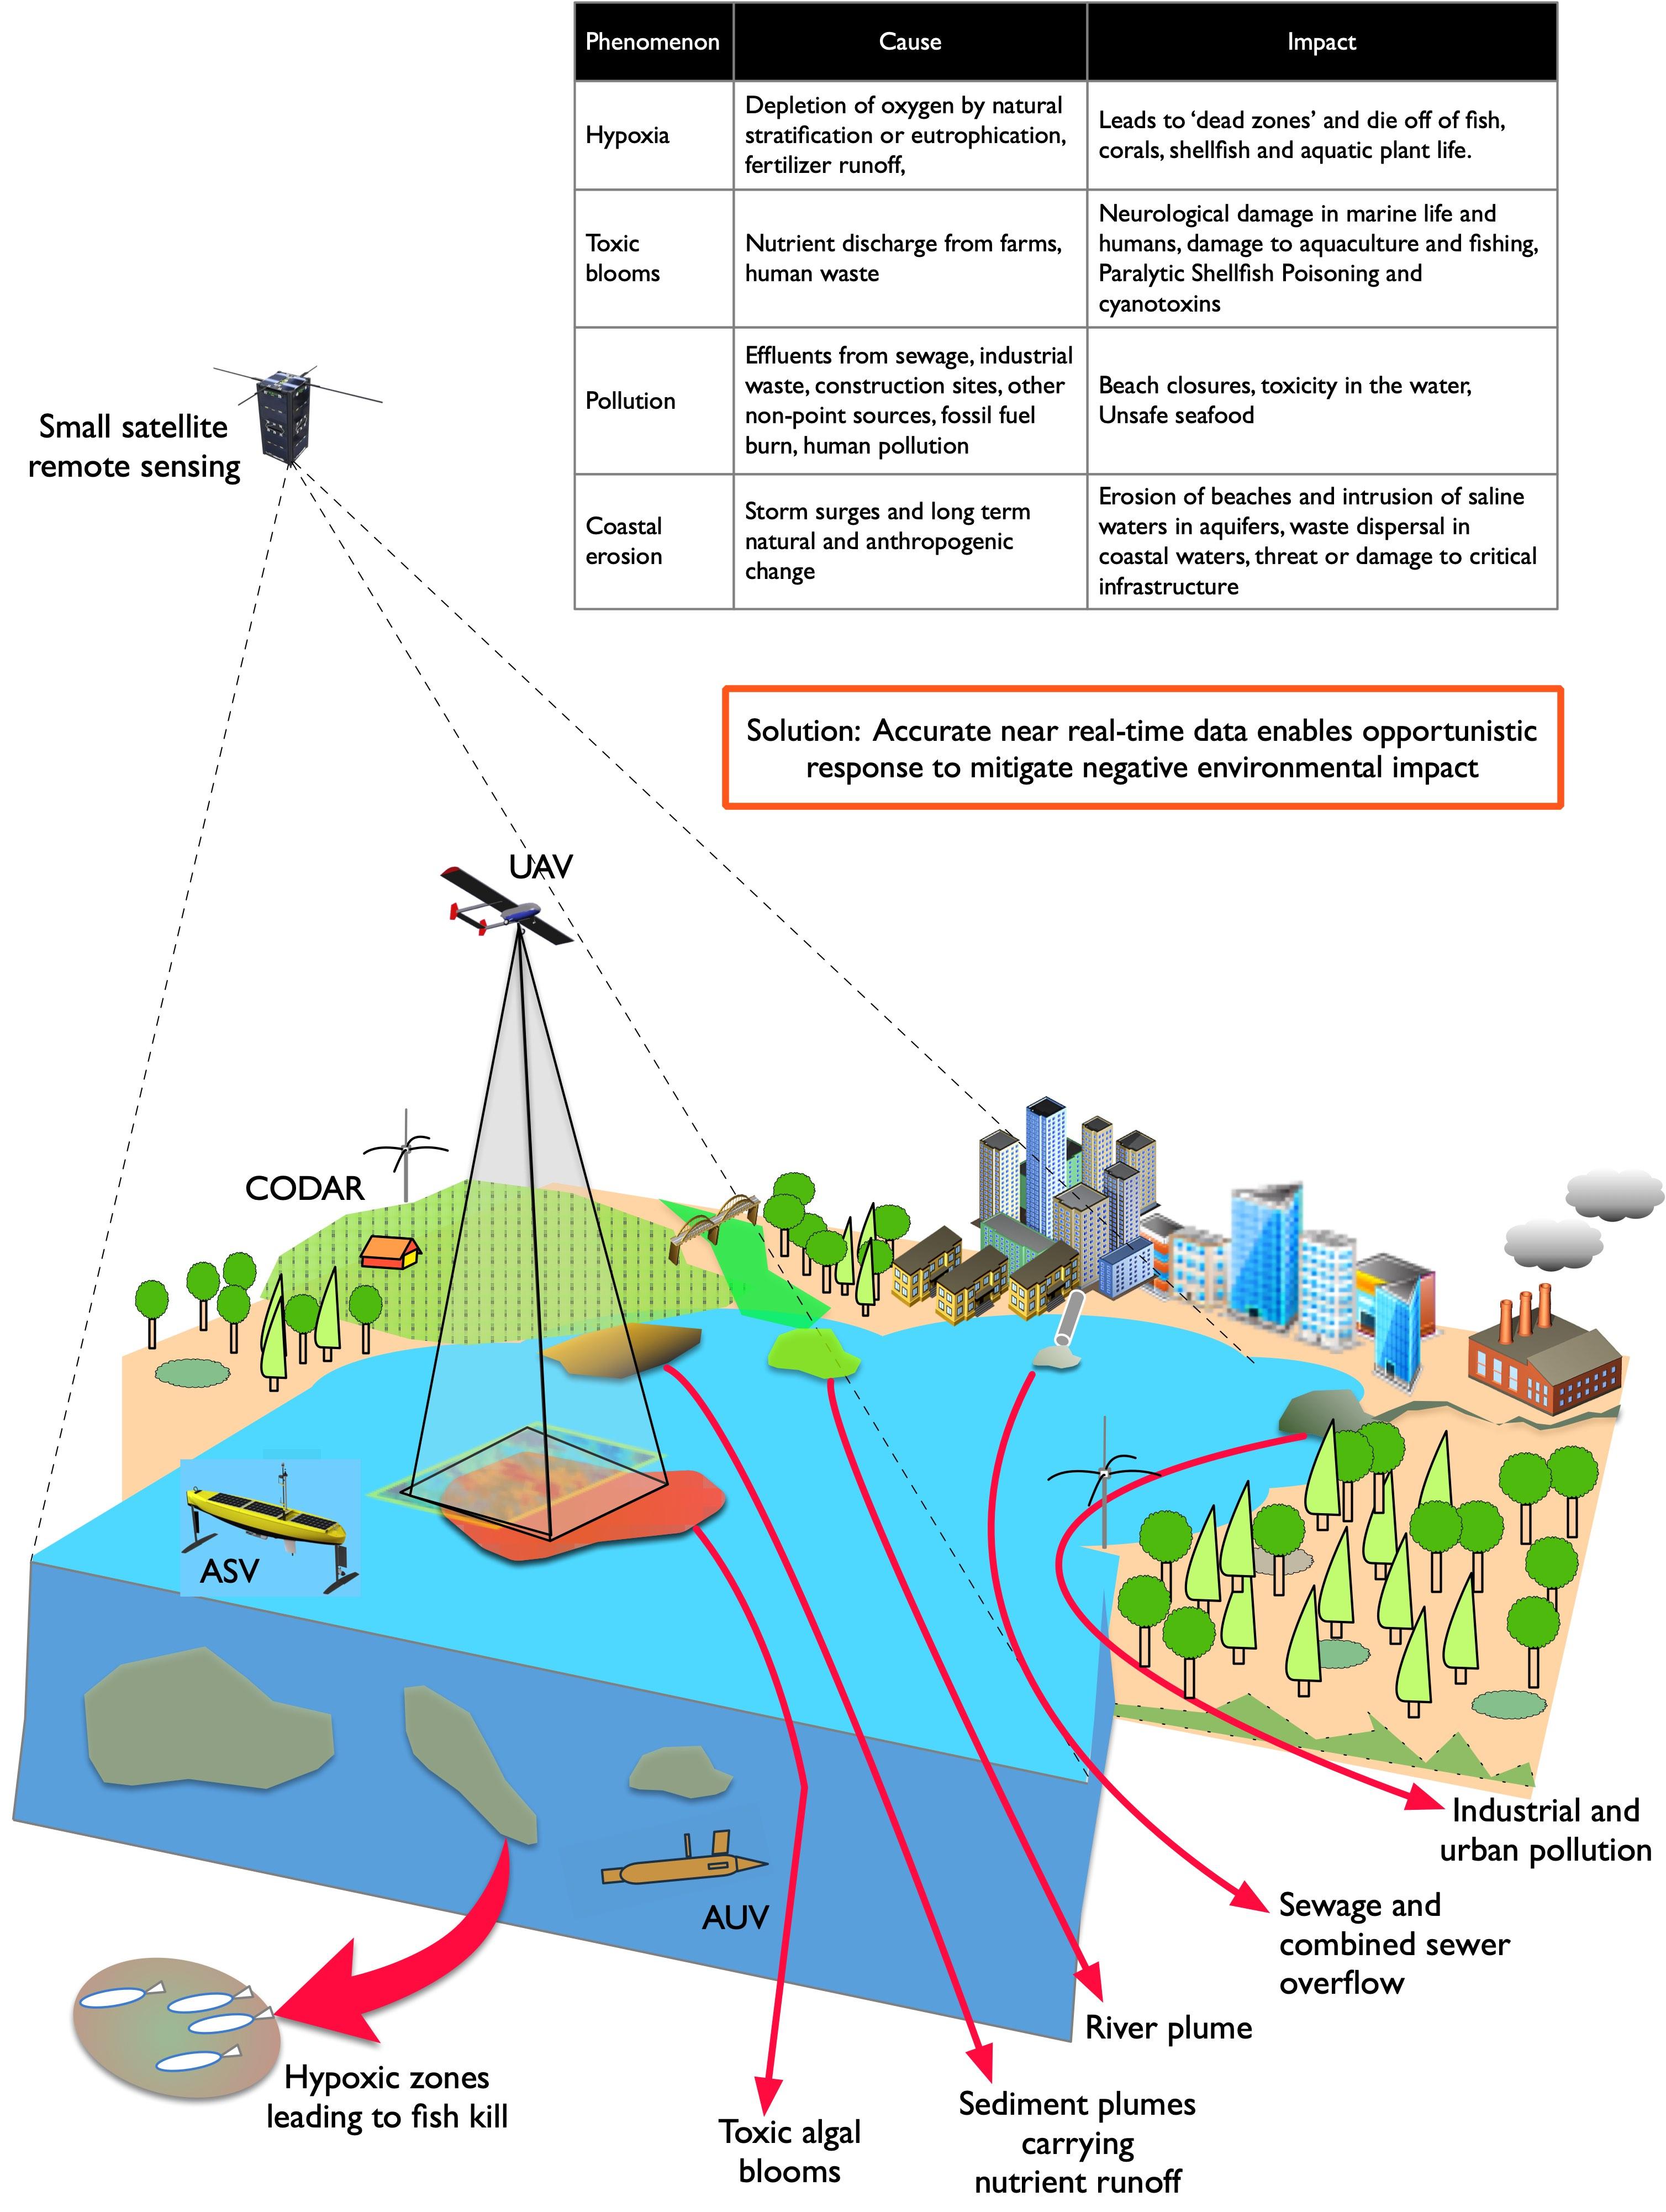
\includegraphics[scale=0.135]{fig/mega-cities-toxic.jpg}
  \caption{Coastal zones are impacted by natural and human-induced
    activities leading to oxygen depleted 'dead' zones, toxic algal
    blooms, pollution, coastal erosion. \pro will use an ensemble of
    small satellites, aerial, surface and underwater vehicles to
    observe the coastal ocean over sustained periods of time to
    provide real-time warning and situational awareness of impactful
    changes to human health, biodiversity and ecosystem services. Note
    the terms UAV: unmanned aerial vehicle, ASV: autonomous surface
    vehicle, AUV: autonomous underwater vehicle, CODAR: Coastal
    High-Frequency (HF) Radar.}
    \label{fig:mega-cities}
\end{figure}

Natural events such as storm surges, tsunamis and upwelled waters
impact such mega-city coastal communities in addition. Turbulence in
the upper water-column with potential injection of nutrients, either
from the benthic or open ocean waters, can often result in sudden
outgrowth of harmful algal blooms, or stirring up human-induced
pollution in such coastal areas.

In both human and nature induced events, the resulting mix can make it
unsafe for any form of human activity often with no obvious and
expected visible sign of near and present danger to local communities.
The consequences can however reverberate with mass scale die-off of
marine life, poisoned shellfish and coastal wildlife and equally
importantly causing neurological damage or fatalities to the human
population on consuming seafood or using beaches for recreation.

Current forms of monitoring are based on sensors (if present) spaced
well apart, periodic human-made measurements that can be impacted by
harsh weather and which typically sub-sample such dynamic coastal
environments.

\pro will integrate state-of-the-art hardware including a small
satellite (\smle) constellation, in situ air, surface and underwater
vehicles with software to control and visualize information derived
from these assets.  The use of \smle's and smart robotic technologies
reduces deployment time to provide opportune solutions and
consequently leverages the latest techniques in AI, Robotics and
software engineering. Coordinated perspectives across different
synoptic spatial and temporal scales in turn will provide a
hyper-realistic situational assessment to stakeholders including those
who drive policy making for human health.

In the report, “Global Marine Trends 2030”, Lloyds Register predicts
that by 2030, the coastal ocean will be “almost unrecognizable”. As we
enter the United Nations “Decade of the Ocean”, \pro will broaden and
deepen knowledge that will aid and augment global ocean sustainability
and stewardship, and the management of our Urban Seas.


% The end user will be a lay person who can obtain near real-time data
% visualized at spatial and temporal scales appropriate to provide
% accurate information to deal with:

% \begin{itemize}

% \item \textbf{coastal pollution} resulting from oil spills, ship
%   discharges, effluents from urban environments resulting in dissolved
%   organics including fecal matter

% \item \textbf{coastal erosion} impacted by steady sea-level rise,
%   storm surges and tsunamis

% \item \textbf{toxic blooms} as a result of naturally occurring
%   phenomenon such as upwelling or anthropogenic nutrient runoff from
%   rivers and creeks passing thru highly fertilized farmland

% \item \textbf{sediment laden plumes} from discharges from rivers and
%   sewage plants emptying into the coastal ocean

% \end{itemize}

\subsection{Why now?}

The oceans cover more than 70\% of the earth's surface. The base of the
human food-chain starts with tiny phytoplankton which generate the
oxygen for every other breadth we take.  With the onset of a climate
crisis, the oceans are changing rapidly in ways we don't
understand. There is an urgent need to develop and deploy new smart
observational methods to provide information at scales that matter to
the 600 million people living along the coast within 10 meters of the
sea level.  Predicting change and providing early warning of hazardous
events, including poor water quality, tainted fish stocks and
intensifying coastal erosion, is essential for the well-being of an
increasingly vulnerable coastal ecosystem and in line with the goals
of the 2021-2030 UN Decade of Ocean Science for Sustainable
Development.

By leveraging rapid advances in technology, \pro will field an
innovative system of small satellites and robust autonomous in-situ
platforms for obtaining unprecedented views of coastal oceans and
atmospheric and land interfaces. We want to aid in the understanding
and monitoring of coastal waters so that they can be explored and
utilized in a sustainable and informed manner.

\pro will therefore enable us, for the first time, to ‘take the pulse’
of the Urban Sea, the primary interface between humans and the
ocean. With the help of a dense robotic network powered by
state-of-the-art integrative software it will deliver actionable
knowledge to stakeholders. In doing so, it will leap-frog the
traditional incremental and siloed methods in ocean observation by
leveraging modern computational methods in data science, autonomous
robotics and smart sensors. The density and diversity of observations
will change by an order of magnitude, the temporal scales of coastal
observations will change from weeks (for traditional shipboard
sampling) or days (for existing satellite data) to hours and minutes
with the provision of real-time information.



% \begin{figure}[H]
%   \centering \subfigure[\pro will build a train of \smle's with a
%   range of sensors to measure explicit ocean variables from
%   space along with marine robots in-situ.]{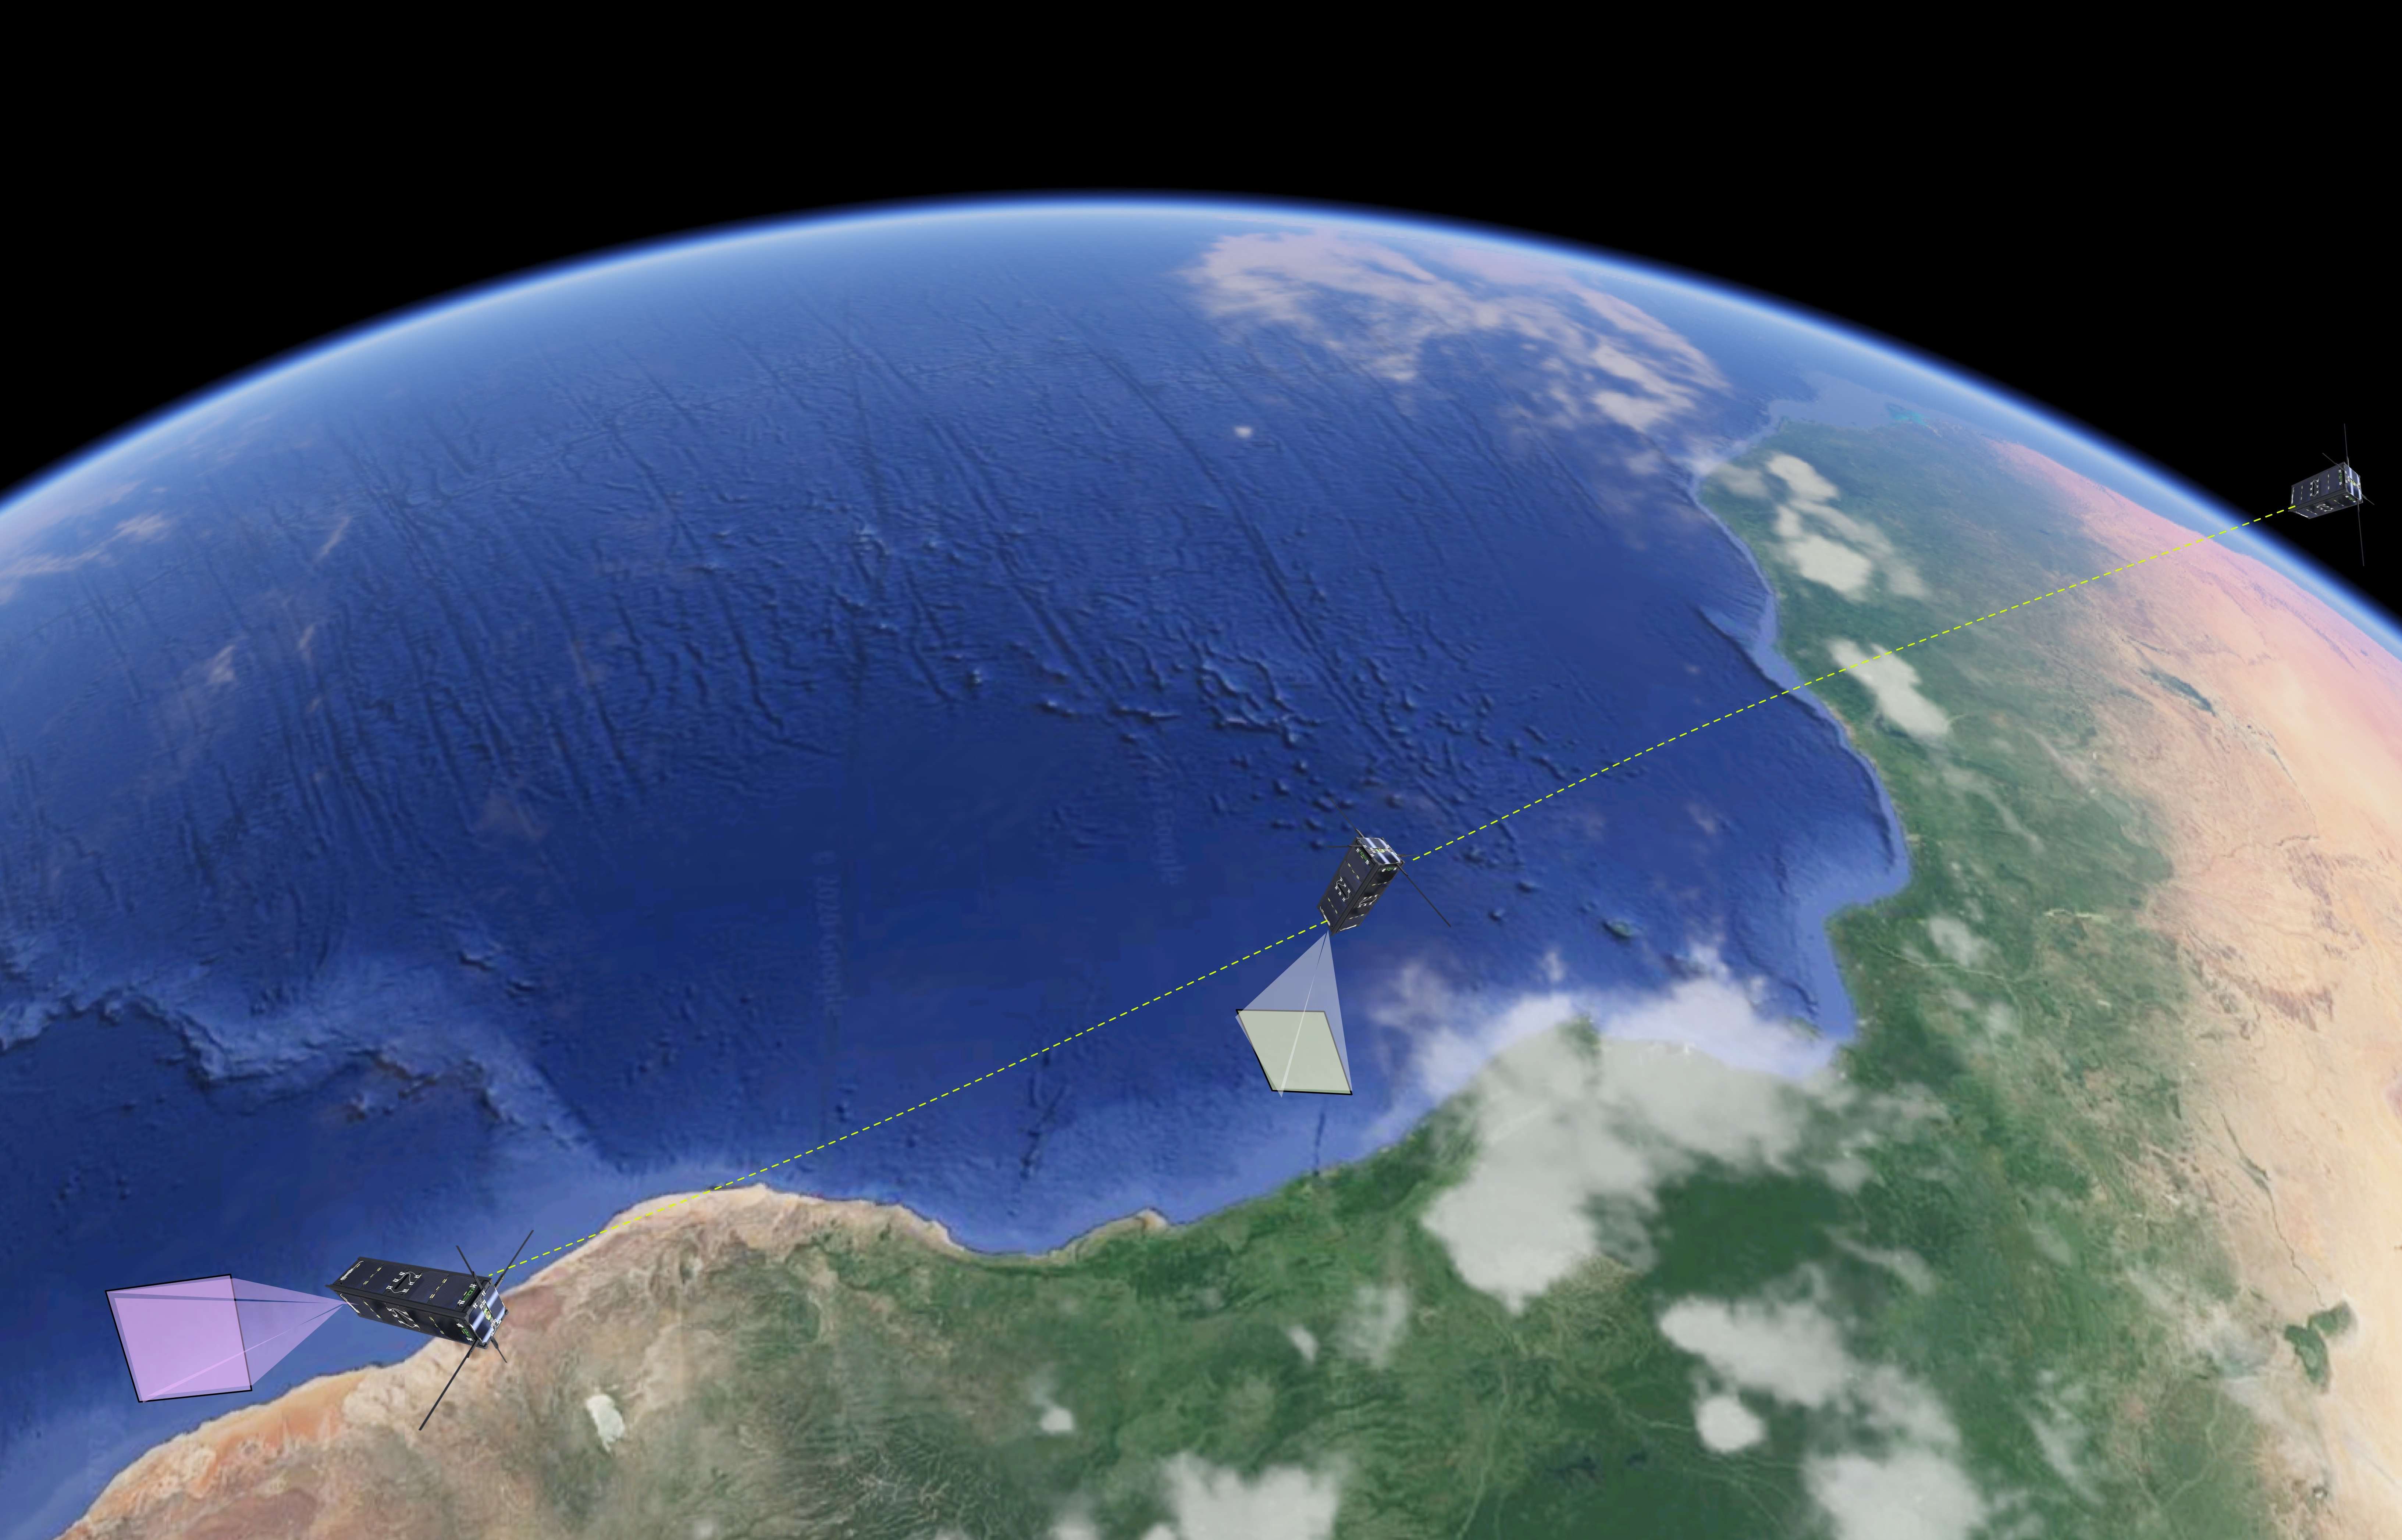
\includegraphics[scale=0.05]{fig/multispace.jpg}\label{fig:multi}}
%   \subfigure[The \pro \emph{Oceanumscope} will provide
%   \emph{persistent, reliable, assimilated} real-time information at
%   scales that matter to the 600 million people living along
%   coasts.]{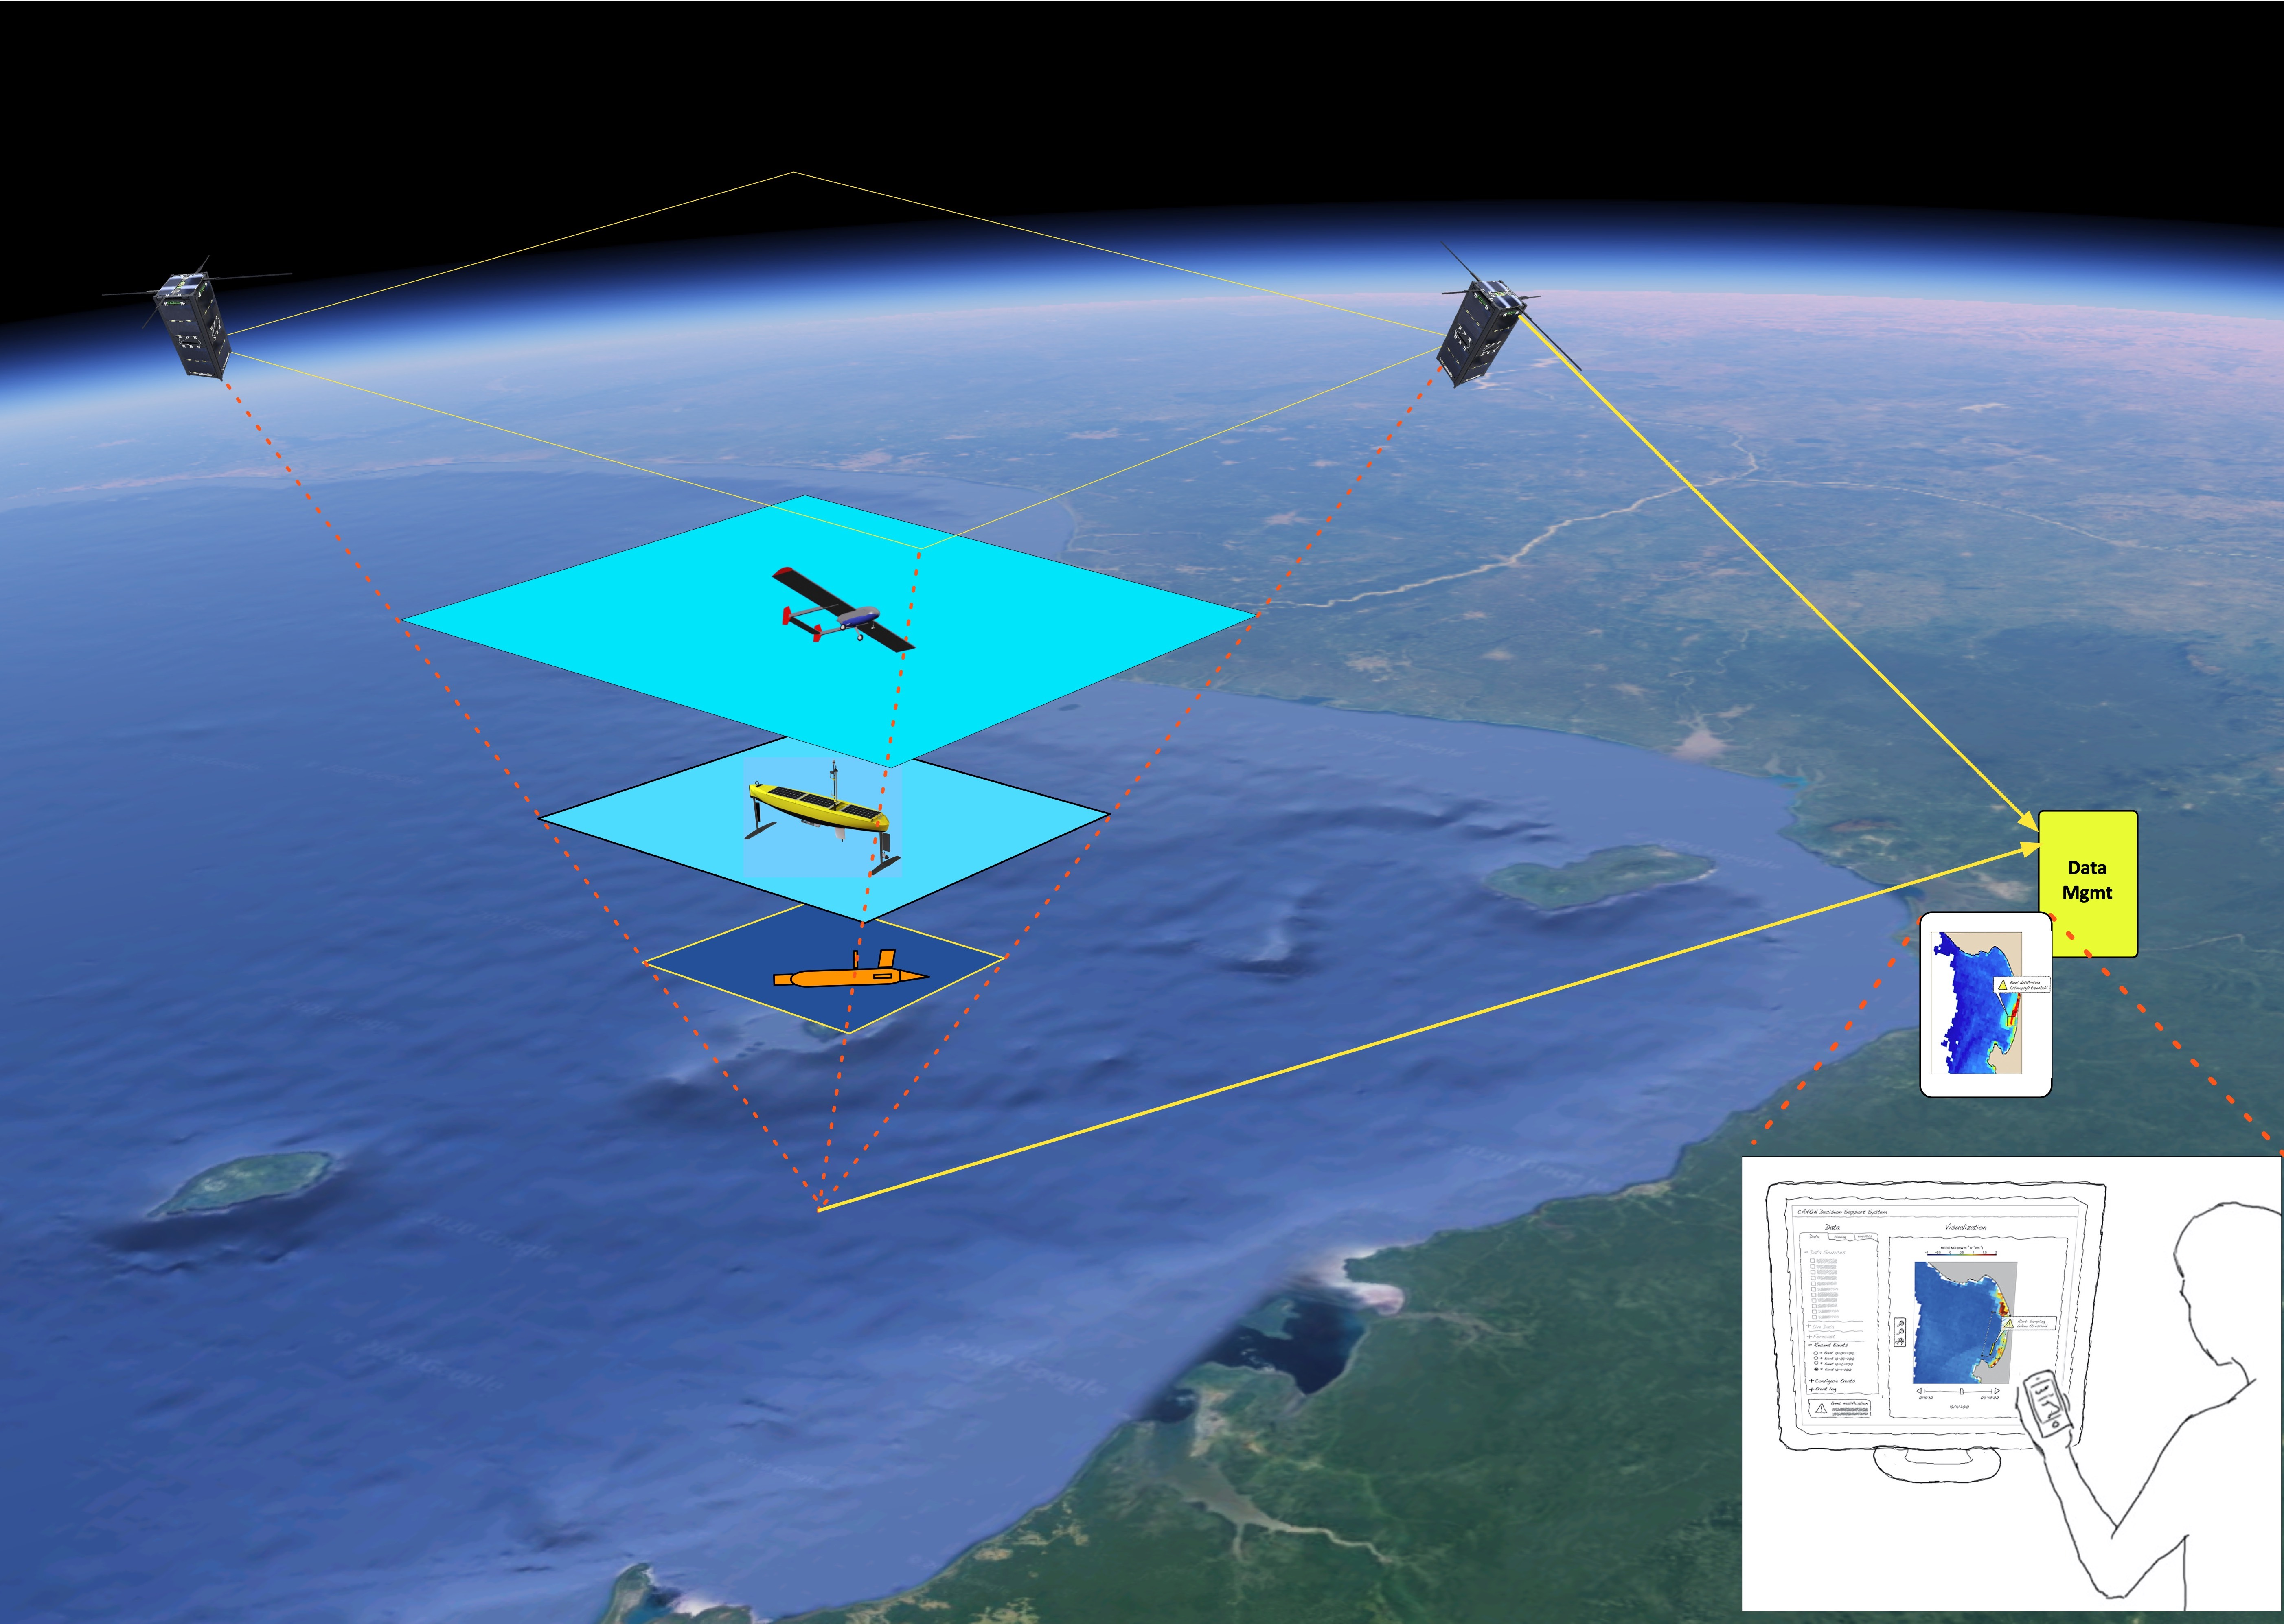
\includegraphics[scale=0.06]{fig/procopio-ensemble.jpg}\label{fig:ensemble}}
%     \caption{\pro is an ensemble of small satellites, aerial, surface
%       and underwater vehicles to observe the coastal ocean over
%       sustained periods of time.}
%   \label{fig:procop}
% \end{figure}


\vspace*{0.1cm}
\subsection{What is the novelty?}

\pro is different from other approaches because it leverages rapid
advances in both hardware and software to provide an end-user with
situational awareness about the coastal ocean, allowing incorporation
of a more holistic approach into decision-making
processes. Mega-cities along the coast have a particularly complex
relationship with the ocean, both dependent on it for recreation and
as a source of food, as well as fearful of its vagaries.

Traditional methods for observing the coastal ocean are inefficient,
not cost-effective, too sparse in space, too sporadic in time or too
localized. In addition, there is poor integration between the various
measurements, especially between those made in-situ and those made by
satellites to produce actionable knowledge for 21\textsuperscript{st}
century decision making.


% Static sensors, or traditional ship-based human-driven sampling, % in
% % the coastal ocean, are not only periodic with rigid schedules. These
% % methods also
% lead to under-sampling the environment at scales, which are inadequate
% to predict large events such as storm surges, coastal erosion, toxic
% blooms, or the advection of coastal pollution.  Equally, the time
% scales which are relevant for action by stakeholders, including those
% who drive policy provided by traditional methods, are inadequate. To
% date, even in developed nations (including the United States), no
% systematic approaches exist that provide synoptic and sub-synoptic
% views of the coastal ocean assimilated in near real-time; mega-cities
% in the developing world are even further behind in being situationally
% aware.

\pro will change that by providing easily accessible information
assimilated from multiple sources of continuous data from space,
aerial, surface and underwater vehicles at scales of resolution
hitherto unavailable. AI will provide correlations between different
events in the air and water-column and result in connections made,
that are nominally difficult or impossible with current methods in
ocean observation. And by doing so, we will technologically leap-frog
the incremental step-by-step approach in aiding vulnerable coastal
communities who rely on the ocean for food, recreation and open
space. \pro will provide the tools to manage environmental, as also
socio-economic issues, allowing solutions beyond the national borders
while responding to emerging global threats.

In the process of providing actionable knowledge, \pro will enable new
modes of management and new understanding about coastal ocean
processes in ways simply not possible before. \pro will allow citizens
to develop a critical understanding of the rapid change taking place
in their Urban Seas and to ‘connect the dots’ between human activity
and the effect on the environment around them. Citizen scientists will
be engaged in generating new observations and new
knowledge. Scientists will be able to pose (and answer) new questions
that could not have been asked before. Policy makers will have the
tools to make informed decisions in time scales that matter, while
developing truly integrative policies on ocean sustainability and
stewardship. PROCOPIO will serve as a replicable blueprint for Ocean
observation in targeting integration, synthesis, cost-effectiveness
and scalability.

While some coastal ocean observatories use a limited number of robotic
assets or remote sensing data, PROCOPIO is unique in the range and
diversity of how these sensors are deployed, how data is integrated
and synthesized, and how citizen engagement is used to improve the
value of the output. PROCOPIO marks a paradigm shift in coastal ocean
observation and in the development of actionable knowledge about the
ocean, by providing information that is accessible and usable by a
wide range of citizenry thus democratizing Ocean knowledge and
overcoming the limitations of traditional approaches.

\begin{enumerate}

\item It opens new vistas of our knowledge of the oceans by providing
  open-data, on-demand, continuous measurements of critical ocean
  variables with unprecedented spatial and temporal resolution.

\item It provides an integrative open-source framework to connect
  robots, services and users in a seamless manner that is both
  scalable and replicable, providing a blueprint for other initiatives
  worldwide.  

\item It leap-frogs current methods by delivering 21st century
  predictive modeling, learning and analytical capabilities, which are
  supported by AI and visualization techniques that are non-existent
  in other interventions.  

\end{enumerate}


\subsection{What will it take?}

The \pro team comes ready with the aerial, surface and underwater
vehicle platforms, together with the extensive suite of software to
provide coordinated observations in the coastal ocean. We will build
custom sensors keyed towards important ocean variables integrated into
a 'train' of \sml platforms.  Such a system working closely with the
in-situ robots will provide a clear consistent set of data
products. This data will be integrated to provide actionable
information to policymakers on the ground as also society in general.

We estimate the total project cost to be about $\sim \$63.5$ Million
over a period of 5 years (2 years for development and 3 for
operational deployment).

% \subsection{Why Gulbenkian?}

% Portugal is an ocean-facing nation that has taken its role in the
% sustainable use of its ocean resources seriously. Within the scope of
% the proposal presented by the Portuguese Government to the UN in 2009,
% the territorial sea, the exclusive economic zone and the continental
% shelf were extended, reinforcing the main assets for the future
% development of the country, and the preservation of marine and coastal
% ecosystems. Further, a direct line can be drawn between the nation's
% historic legacy of ocean exploration to the dominance of \ls at \univ
% at the cutting edge of autonomous robotic marine platforms. We believe
% it is not only relevant but critical that this momentum on its
% intellectual landscape be maintained in service of science and
% society. And sourced within Portugal.

% More importantly this project is aimed directly at the core of the
% Gulbenkian Foundation's focus on sustainability, knowledge, climate
% change and the rise of inequality. By working with developing nations'
% coastal meg-cities we aim to directly target our inter-disciplinary
% work at a critical problem of immense societal interest, namely the
% future of our oceans. 

% \subsection{Where will it be built?}

% With the extensive experience \vig has in building \smle's and the
% significant marine robotic assets in nearby \unive, we expect to
% design, build and test the \smle's in Vigo, Spain and operate the
% \smle's along with the marine robotic assets from an \texttt{Ocean
%   Space Center} in Porto. Oceanographers from the US, Portugal, Spain
% and other EU nations will provide significant guidance on mission
% concepts and data assimilation, will all sensor software development
% and integration taking place in Porto, Portugal. The latter city has
% multiple non-stop flights from the US every day for US scientists,
% including those on the team to participate in the design, construction
% and operation, both virtually and in-person.

\subsection{Governance}

The governing board of \pro will consist of prominent strategic
advisors from the US, including stakeholders and funders. In addition,
the project principals will be aided and advised by a scientific
advisory board (\texttt{SAB}) consisting of technologists, ocean going
scientists, ecologists and policy makers from the US, Europe and
targeted coastal states.

\subsection{The Team}

\proe’s inter-disciplinary team of seasoned researchers (see bio's
below) from the universities of Columbia/US, Porto/Portugal and
Vigo/Spain have worked in all the major oceans, fielded tens of robots
at sea simultaneously, designed/built/flown and operated multiple
\smle's and complex systems in the deep sea and deep space.
% Mars. % \pro will
% build on these efforts and experience, augmented by new sensors,
% hardware and software to develop the first portable 
% \emph{Oceanumscope}.


% There is a pressing need for a sustained, persistent, and affordable
% presence in the oceans to help us understand and monitor how key
% processes such as acidification, hypoxia, toxic blooms, pollution,
% erosion (amongst others) are impacting global ocean sustainability and
% stewardship. Traditional ship or remote-sensing methods are neither
% cost-effective nor provide assimilated real-time information across
% adjustable spatio-temporal scales. They also require extensive human
% support and exposure to the harsh environment of the ocean. The lag
% between processed data and \emph{information} available to
% stake-holders is substantially long to void any form of environmental
% situational awareness.

% Conversely, technological change has put within our reach, the ability
% to sense the environment, process and visualize data in ways hitherto
% not possible.
% The information and robotics revolutions have rapidly
% advanced making such an exploration loop realistic and viable
% cost-effectively.
% Data can be gathered, uploaded to the cloud, rapidly processed and
% analyzed using techniques in Machine Learning and Data Analysis that
% barely existed a few years ago. Stunning visuals which enhance our
% knowledge of the environment, can rapidly be put together to provide
% stake-holders such as policy-makers and NGO's \emph{actionable} ways
% to respond to hazardous events such as tainted fish stocks, coastal
% erosion, storm surges and inclement ocean weather for subsistence
% fishermen.

% We believe that with the help of coordinated observations from space,
% aerial, surface and underwater vehicles, guided by Artificial
% Intelligence (AI), researchers can rapidly process and assimilate data
% from multiple sources such as satellite remote sensing, shore-based
% radar and mobile and immobile robots amongst others. In doing so, we
% would provide persistent and reliable oceanographic observations
% across space and time.

% While there are many large telescopes looking at the heavens; yet no
% consistent observational system looking at and into our oceans,
% exist. We will build such a rapidly deployable, multi-domain, portable
% robotic observatory, to observe our endangered coastal waters. \pro
% will be that observatory.

% Traditional ship or remote-sensing methods are neither cost-effective
% nor provide assimilated real-time information across adjustable
% spatio-temporal scales. \pro will leverage rapid advances in
% technology to field an innovative system of student-built small
% satellites and robust autonomous in-situ platforms to make a massive
% “microscope” to obtain unprecedented views of coastal areas and of its
% atmospheric and land interfaces. In doing so, it will aid in urgently
% understanding and monitoring coastal waters, as well as to explore and
% exploit them in a sustainable and informed manner.



\newpage
\vspace*{0.5cm}
\section{Brief Bios of the Principals}



\parbox{6.25in}{
\begin{wrapfigure}{r}{0.45\textwidth}
  \centering
  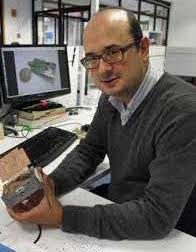
\includegraphics[width=.75\linewidth]{fig/FAguado.jpg}
\end{wrapfigure}
\textbf{Fernando Aguado} is an Associate Professor at the University
of Vigo. He was the principal investigator (PI) of the Xatcobeo
cubesat, the first Galician satellite and first Spanish Cubesat. He
was also the PI of HUMSAT-D and sector B of Serpens (both developed
within the Basic Space Technology Initiative of UN with the support of
ESA) and the LUME-1 \smle. He has coordinated the design, manufacturing
and integration of various Cubesats for maritime and airplane tracking
applications as well as for machine to machine communications.
\\
\textbf{email: }\emph{faguado@tsc.uvigo.es} \\
\textbf{Web: }\url{https://bit.ly/3avJlwX}\\
}

% \vspace*{+0.1in}

\parbox{6.25in}{
\begin{wrapfigure}{r}{0.45\textwidth}
  \centering
  \includegraphics[width=.75\linewidth]{fig/Krajan.png}
\end{wrapfigure}
\textbf{Kanna Rajan} holds faculty appointments at the \univ \&
\univne, Norway in autonomous systems. He spent 10 years at \inst
where his software was responsible for the command/control of the 1999
New Millennium Deep Space 1, 65 Million miles from Earth and the 2003
Mars Exploration Rovers mission on the Red Planet. In 2005 he moved to
\mba and built the only AI group in marine robotics. His field work
and publications have been in highly ranked peer-reviewed publications
including \emph{Science}, Intnl. Journal of Robotics Research, the AI
Journal and Journal of Field Robotics. He has participated in
scientific oceanographic cruises in the Pacific and Atlantic.
\\
\textbf{email: }\emph{Kanna.Rajan@fe.up.pt}\\
\textbf{Web:
}\url{https://www.ntnu.edu/employees/kanna.rajan}}\footnotemark\footnotetext{Principal
point of contact}

\newpage
% \vspace*{0.5cm}

\parbox{6.25in}{
\begin{wrapfigure}{r}{0.45\textwidth}
  \centering
  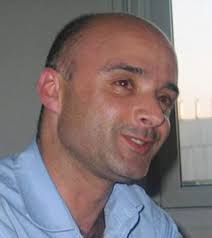
\includegraphics[width=.75\linewidth]{fig/JBS.jpg}
\end{wrapfigure}
\textbf{Jo\~ao Sousa} is a Professor at the Faculty of Engineering,
Univ. of Porto, Portugal and the head of the Underwater Systems and
Technology Laboratory (\lse). The lab has pioneered the design,
construction and deployment of networked underwater, surface and air
vehicles for applications in ocean sciences and defense and is at the
vanguard of operations of coordinated aerial, surface and underwater
vehicles. The lab designed the award-winning Light Autonomous
Underwater Vehicle and the \ls open source software for networked
vehicle systems, and has been key in organizing large scale
experiments, including the annual Rapid Environmental Picture (\rpe)
organized jointly with the Portuguese Navy since 2010. He has
participated in numerous engineering and scientific oceanographic
cruises.
\\
\textbf{email: }\emph{jtasso@fe.up.pt}\\
\textbf{Web: }\url{https://bit.ly/2J6cKCc}}
% {https://lsts.pt/member/jo%C3%A3o-sousa}


\vspace{+0.25in}
\parbox{6.25in}{
\begin{wrapfigure}{r}{0.45\textwidth}
 \centering
  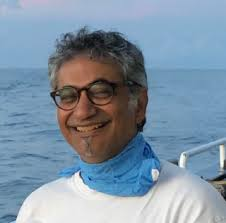
\includegraphics[width=.75\linewidth]{fig/ASub.jpg}
\end{wrapfigure}

\textbf{Ajit Subramaniam} is a Lamont Research Professor at the
Lamont-Doherty Earth Observatory (\ldeoe) of Columbia University, New
York.  He is an oceanographer who uses knowledge of remote sensing,
ocean optics, phytoplankton physiology, biological and physical
oceanography and geographical information systems to better understand
how the marine ecosystem functions and can be managed.  He has worked
for National Oceanic and Atmospheric Administration (NOAA), and held
appointments at the Univ. of Maryland and the Univ. of Southern
California prior to moving \ldeo in 2004. He has served as the Program
Director for the Marine Microbiology Initiative at the Gordon and
Betty Moore Foundation and a program manager in the Biological
Oceanography Program at the U.S. National Science Foundation (NSF). He
has participated in oceanographic cruises in all parts of the world.
\\
\textbf{email: }\emph{ajit@ldeo.columbia.edu} \\
\textbf{Web: }\url{https://www.ldeo.columbia.edu/~ajit/}
}

\end{document}

